\subsection{Top hatch}
The top hatch is at the top of the arc chamber, it has only 35 cm diameter,
which is a challenge when thinking about using it as a robotic system access
point. Furthermore its proximity to the blades and the free space outside the
arc chamber create interesting possibilities for its use.
%Essa escotilha localizada no topo do aro câmara possui uma abertura de apenas
%35 cm de diâmetro, o que cria um desafio quando se pensa em utiliza-la como
%ponto de acesso para um robô. Por outro lado sua proximidade às pás e a área
% livre fora do aro câmara criam possibilidades interessantes para seu uso.

\textbf{Advantages}
\begin{itemize}
  \item robot fixation stability
  \item reference point, facilitating localization system, mapping, control and
  calibration
  \item built logistics: conveyor gantry to position the robot and the
  HVOF system
\end{itemize}

\textbf{Disadvantages}
\begin{itemize}
  \item difficulty in finding robots of such size (35 cm diameter)
  \item during the operation, the robot must be
  removed to rotate the blades
  \item not a general solution, specific to Jirau
\end{itemize}

The simplest solution to this access is to use an industrial robotic manipulator.
The choice of the commercial robot is primarily associated within reach. On the
other hand, only a small share of commercial robots have the dimension to fit
the top hatch. Thus, the study was focused on the KUKA Light Weight (LBR
iiwa 14 R820), robot whose base diagonal is less than 35 cm.

%A solução mais simples para este acessso é a utilização de um robô industrial
%comercial. A escolha do robô está primariamente associada ao seu alcance. Por
% outro lado, apenas uma pequena parcela dos robôs comerciais possuem a dimensão necessária para
%atravessar a escotilha. Sendo assim, o estudo foi direcionada para o uso do
%KUKA Light Weight (LBR iiwa 14 R820), robô cuja diagonal da base é inferior aos
%35 cm da escotilha.


The LBR R820 weights 30 kg, has seven joints and has 14 kg payload, enough to
carry the coating equipment. However, further studies are needed to validate
the robot, as the speed and precision requirements when coating.

%O LBR R820 pesa 30 kg, possui 7 eixos e suporta carga de 14kg,
%suficiente por uma pequena margem para carregar o equipamento de
%revestimento. Entretanto, são necessários estudos aprofundados para valida-lo,
%como os requisitos de velocidade e precisão quando percorrendo a trajetória
%para a realização do revestimento.

To place the LBR R820 in a position where it is able to process all the
blade, a hinged base model was proposed. The base consists of two telescopic
links interconnected by a revolute joint, and the first link is attached to the
top hatch itself. To cover the entire blade, the base must be able to assume different angles with
respect to the insertion axis, and the links must be telescopic type, with
prismatic joints, positioning sensors, and recirculating ball actuators for low
backlash and high precision. 

The base's structure would consist of cylinders with maximized diameter and
small thickness, which features a high polar moment of inertia and light weight,
providing great bending stiffness and minimizing positioning errors and
excessive vibration. Figure~\ref{fig::base_recolhida} and
figure~\ref{fig::base_extendida} show the manipulator' base concept in two
configurations: retracted and extended.

%A base consiste em 3 braços
%telescópicos que permitem a extensão do sistema para prover o alcance
%necessário ao manipulador e o recolhimento para uma configuração incial que
%permita a entrada do manipulador no aro câmara com segurança, sem o risco de
%choques ou interferências indesejadas. Além disso, uma junta rotativa oferece
% mais um grau de liberdade para o sistema, facilitando o acesso do manipulador à toda ar
%superfície da pá. 

%Os atuadores da base são acionados eletricamente e possuem sensores de
%posicionamento. Atuadores de esferas recirculantes foram escolhidos devido à
%baixa folga e precisão elevada. A estrutura da base é composta por cilindros de
%diâmetro maximizado e pequena espessura, o que oferece um momento de inércia
%polar elevado e baixo peso, fornecendo grande rigidez à flexão e minimizando
%erros de posicionamento e vibração excessiva. A
% figura~\ref{fig::base_recolhida} e a figura~\ref{fig::base_extendida} apresentam o conceito da base do manipulador em duas configurações: recolhida (configuração
%de entrada) e estendida (configuração de operação).

\begin{figure}[h!]
\centering
	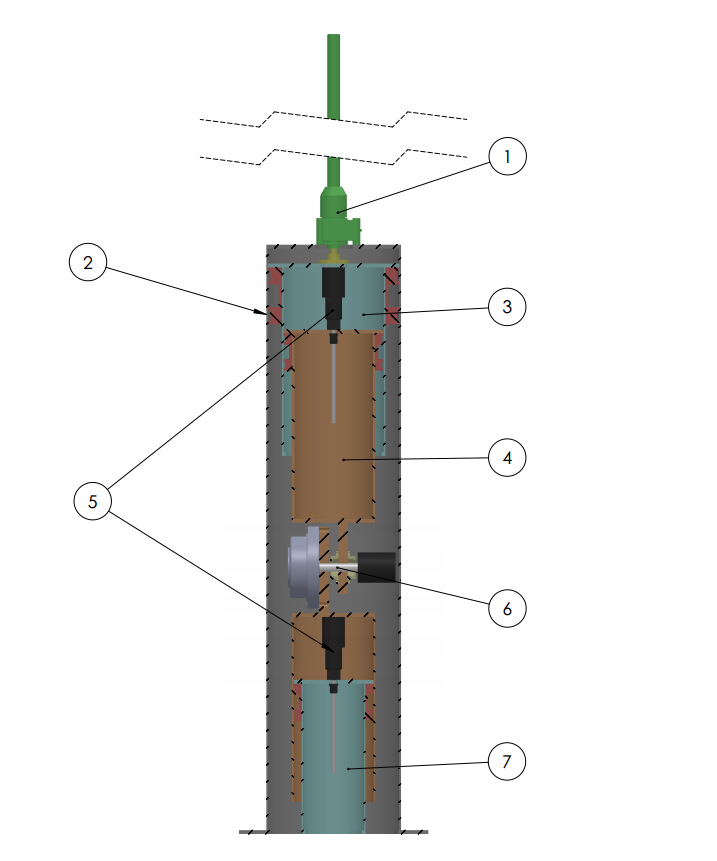
\includegraphics[width=\columnwidth]{figs/estudo/solid/Base_Recolhida.PNG} 
	\caption{Initial configuration of the base (retracted)}
	\label{fig::base_recolhida}
\end{figure}

\begin{figure}[h!]
\centering
	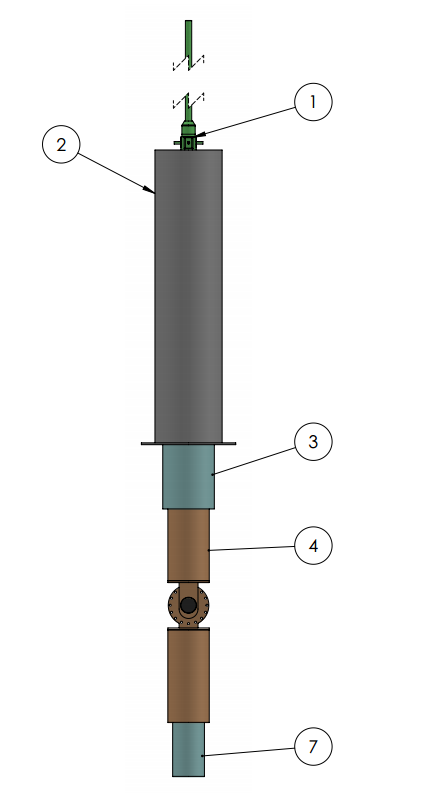
\includegraphics[width=\columnwidth]{figs/estudo/solid/Base_Extendida.PNG} 
	\caption{Base on extended configuration}
	\label{fig::base_extendida}
\end{figure}

The main components of the base are shown in figures~\ref{fig::base_recolhida}
and~\ref{fig::base_extendida}: 1) Linear actuator gear worm;
2) fixed base; 3) prismatic arm \#1; 4) Arm Prismatic \#2; 5) linear actuators;
6) revolute joint; 7) prismatic arm. Figure~\ref{fig::base_ambiente3d_recolhida} shows the base and KUKA LBR
R820 manipulator.

%Os componentes principais da base estão representados nas
%figuras~\ref{fig::base_recolhida} e~\ref{fig::base_extendida}, são: 1) atuador
%linear por sem-fim coroa; 2) base fixa; 3) braço prismático \#1; 4) braço
%prismático \#2; 5) atuadores lineares; 6) junta rotativa; 7) braço prismático
%\#3.

%A figura~\ref{fig::base_ambiente3d_recolhida} demonstra a base com o
%manipulador KUKA LBR 820 e as dimensões extremas, em milímetros, estimadas para
%% o interior e para fora da turbina, na configuração inicial de entrada no aro
%câmara pela escotilha superior.
%A figura~\ref{fig::base_ambiente3d_extendida} apresenta a base com o
% manipulador em uma configuração qualquer de operação, demonstrando o ganho de alcance e
%generalidade de posicionamento fornecidos pela base.

\begin{figure}[h!]
\centering
	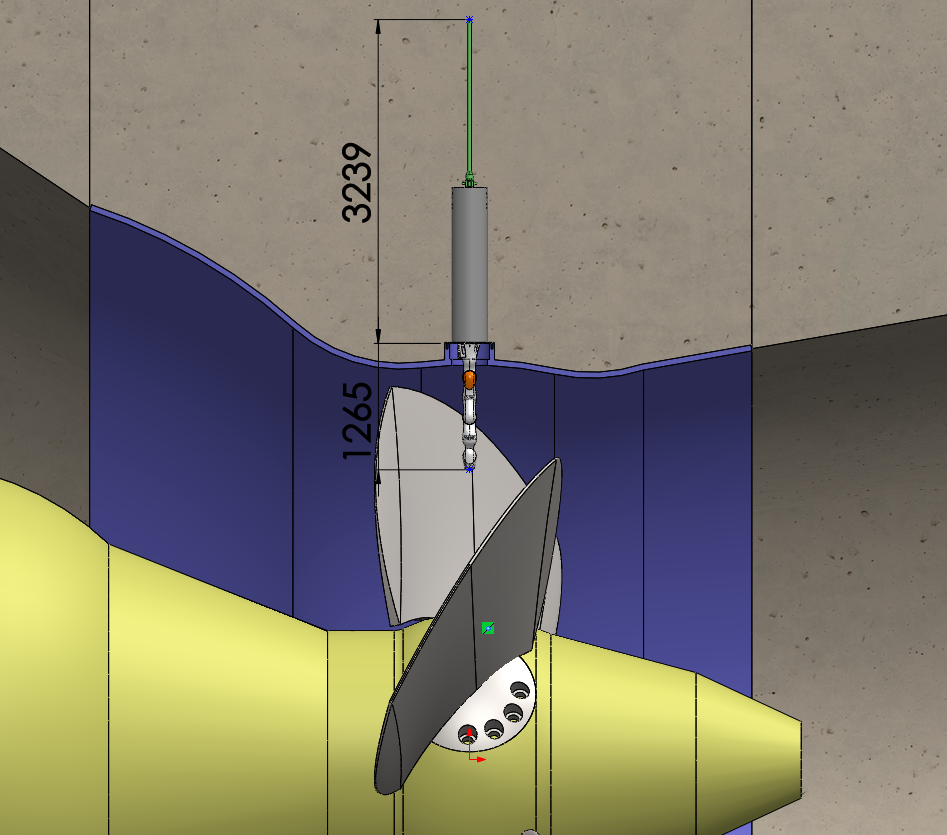
\includegraphics[width=\columnwidth]{figs/estudo/solid/Base_Ambiente3d_Recolhida.png} 
	\caption{Base and KUKA LBR R820 manipulator}
	\label{fig::base_ambiente3d_recolhida}
\end{figure}

%\begin{figure}[h!]
%\centering
%
	% 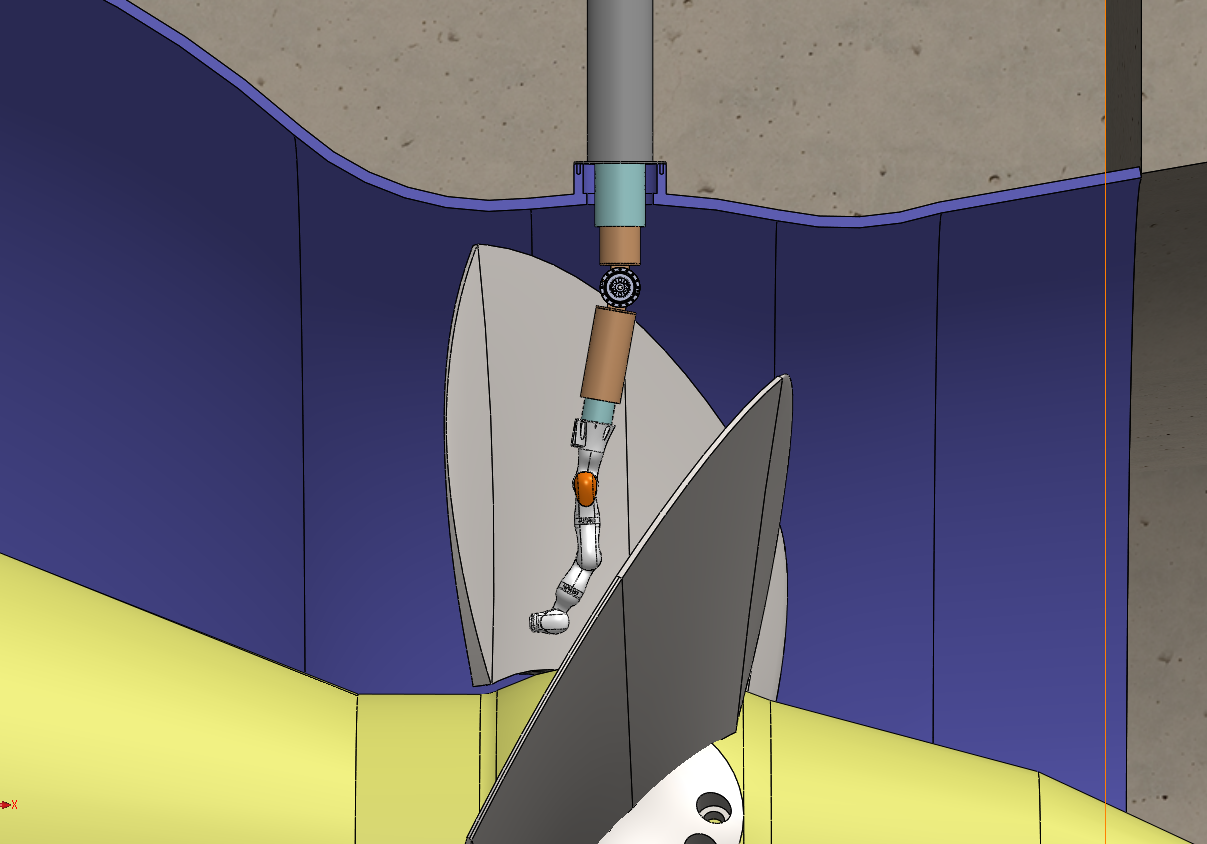
\includegraphics[width=\columnwidth]{figs/estudo/solid/Base_Ambiente3d_Operacao.PNG}
%	\caption{Base em uma geral configuração de operação}
%	\label{fig::base_ambiente3d_extendida}
%\end{figure}


%Tendo como objetivo posicionar o LBR R820 em uma posição onde seja capaz de
%trabalhar toda a pá, um modelo de base articulada foi proposto. A base
%composta de dois elos interligados por uma junta de rotação é fixada na
%própria escotilha. Para que seja possível cobrir toda a pá,
%a base deve ser capaz de assumir diversas angulações com respeito ao
%eixo de inserção, e a junta que conecta os dois segmentos da base também
% precisa ter sua posição alterada, o que pode ser realizado manualmente ou com atuador.

Inserting the system, composed of the base and manipulator, in the top
hatch access requires special care, as the system total length is greater
than the distance from the top of the arc chamber to the turbine nose. Thus,
the arm and the base will need to be rotated during the insertion process,
which will result in misalignment of the central mass (with respect to the axis
perpendicular to the hatch) and will require a guide to compensate the torque
generated by such misalignment.

%Introduzir o robô, composto pelo conjunto base-LBR R820, é uma tarefa cuidadosa
%pois a extensão total será maior que a distância do topo do aro câmara ao
%cone da turbina. Ou seja, o braço e a base precisarão ser rotacionados
%durante o processo de inserção, o que acarretará no desalinhamento do centro de
%massa (com relação ao eixo perpendicular à escotilha) e exigirá uma guia para
%resistir ao torque gerado por esse desalinhamento.


As the system is attached to the top hatch and the joint base is fixed,
the torques are expected to be less than 3000 Nm on jointe base, and 4000 Nm on
the base during coating operation.

%Com o robô fixado na escotilha e a junta da base travada, são esperados torques
%inferiores a 3000 Nm sobre a junta e 4000 Nm sobre a base, durante a operação
% de revestimento.

%Ao se avaliar as possibilidades de realizar o revestimento sem a necessidade de
%placas de sacrifício, percebe-se que poderá ser realizado se a junta da
%base estiver paralela à pá (que para efeito de cálculo foi assumida com uma
%angulação de $45^o$ com relação ao eixo da turbina). Para esse caso a junta
% precisa realizar uma rotação à velcidade mínima de 34 rad/min. Essa velocidade possibilita a
%pistola de revestimento percorrer verticalmente a pá sem pausa. Percorrer
%horizontalmente a pá não será possível devido às restrições nas dimensções da
%base. O cálculo foi realizado por um estudo puramente geométrico, utilizando as
%informações reais de extensão da pá e área de trabalho do robô, assumindo um
%modelo simples da pá, sem curvatura.

